\section{Metodología}

En este capítulo se presenta la descripción los datos utilizados para el desarrollo del trabajo, y se presenta la descripción de un modelo de caminata aleatoria, un modelo lineal, y uno de redes neuronales artificiales; todos empleados para el pronóstico del tipo de cambio. Además se introducen las medidas de error de pronóstico utilizadas para su comparación y la interpretación de los parámetros obtenidos en la red neuronal. Se sigue una metodología cercana a la presentada por \textcite{sunythesis}, replicando los resultado para el caso de Guatemala y Estados Unidos.

% Cuáles son las variables importantes para el modelo y de dónde se obtuvieron
\subsection{Variables relevantes}
Para el desarrollo del trabajo se escoge el modelo monetario de precios rígidos (SPMM, por sus siglas en inglés) para su estimación, donde las variables independientes explican los movimientos del tipo de cambio del quetzal contra el dólar estadounidense.

\subsubsection{Variable dependiente}
Como variable explicada por los modelos de pronóstico se tiene el logaritmo natural del tipo de cambio \textit{spot} del quetzal en relación con el dólar estadounidense.

\subsubsection{Variables independientes}
Las variables independientes de acuerdo con el SPMM son: 

\begin{itemize}
	\item Logaritmo natural de la oferta relativa de dinero entre Guatemala y Estados Unidos.
	\item Logaritmo natural del producto interno bruto (PIB) relativo.
	\item El diferencial de las tasas de interés.
	\item El diferencial de la inflación.
\end{itemize}


% De dónde se obtuvieron los datos y en qué forma se utilizaron
\subsection{Descripción de los datos}
\label{subsec:descdatos}
Para el ajuste de los modelos se utilizan datos mensuales desde enero de 2001 hasta diciembre de 2015, lo que conforma un total de 180 observaciones. Los datos fueron obtenidos del Sistema de Información Macroeconómica y Financiera de la Región (SIMAFIR) de la Secretaría Ejecutiva del Consejo Monetario Centroamericano (SECMCA) y de la base de datos de estadísticas financieras internacionales (IFS, por sus siglas en inglés) del Fondo Monetario Internacional.\\

La muestra de estimación comprende las observaciones desde enero de 2001 hasta diciembre de 2012 (para un total de 144 observaciones), mientras que la muestra para el pronóstico comprende las observaciones desde enero de 2013 hasta diciembre de 2015 (para un total de 36 observaciones), de tal forma que el pronóstico del tipo de cambio mensual se realiza para un corto y mediano plazo.\\

La descripción de los datos es la siguiente:

\begin{itemize}
	\item Tipo de cambio \textit{spot}: promedio mensual del tipo de cambio de referencia en quetzales por dólar, obtenido del SIMAFIR. Se utiliza el logaritmo natural.
	
	\item Oferta de dinero: mensual del agregado monetario M2 para Guatemala y Estados Unidos en sus monedas correspondientes. Obtenido del SIMAFIR para Guatemala, y del IFS para Estados Unidos. La serie se utiliza como índice, tomando como observación base enero del 2001 (que tiene un valor de 100).
	
	\item PIB real: trimestral con base en enero de 2001 obtenido del SIMAFIR y convertido a mensual a través del índice de actividad económica (IMAE) utilizando un promedio ponderado. Serie trimestral del PIB nominal de Estados Unidos, obtenido del IFS e interpolado mensualmente. Finalmente se deflacta con el índice de precios al consumidor para Estados Unidos, con base en enero de 2001. Los datos se utilizan como índices, con base en enero de 2001 y un valor de 100.
	
	\item Tasas de interés de corto plazo: mensual del SIMAFIR para Guatemala, utilizando la tasa pasiva en moneda nacional. Para Estados Unidos el promedio mensual de la tasa de interés en el mercado de dinero, obtenida del IFS.
	
	\item Tasa de inflación esperada: mensual calculada como el porcentaje de cambio intermensual en el índice de precios al consumidor de Guatemala y Estados Unidos, ambos con base en enero de 2001.
	
\end{itemize}

\subsection{Herramientas para estimación}

Se utiliza el software EViews 9 para correr el modelo de regresión lineal, en el cual se puede correr la regresión, obtener los resultados, y realizar algunas pruebas de diagnóstico. Para el trabajo realizado con la red neuronal se trabaja con el lenguaje de programación y estadística \textit{R}, en el cual se efectúa la normalización de los datos y el entrenamiento de la red neuronal utilizando el paquete \textit{neuralnet}.

% Sobre el modelo de caminata aleatoria
\subsection{Modelo de caminata aleatoria}
Como punto de referencia para comparar los resultados obtenidos por el modelo monetario en su versión lineal y no lineal, y siguiendo la metodología de \textcite{meese1983empirical}, se propone un modelo de caminata aleatoria de la forma: 

\begin{equation}
	s_t = s_{t-1} + \epsilon_t
\end{equation}

donde $s_t$ es el tipo de cambio \textit{spot} del quetzal contra el dólar en el tiempo $t$, en su forma de logaritmo natural, y $\epsilon_t$ es un proceso de error estocástico.En el trabajo, los pronósticos del tipo de cambio sobre la parte reservada de la muestra se generan con el modelo de caminata aleatoria tomando el último dato observado, y sumando una componente aleatoria $\epsilon_t \sim \mathrm{Normal}(0, \sigma_e^2)$, donde $\sigma_e^2$ es la varianza de las observaciones dentro de la muestra\footnote{En adelante las referencias ``dentro de la muestra'' se refieren a la muestra de estimación descrita en la sección \ref{subsec:descdatos}.}.

% Sobre el modelo simple de regresión lineal aplicado al modelo monetario
\subsection{Modelo de regresión lineal}
\label{subsec:modeloLineal}

Se utiliza un modelo macroeconómico lineal $\Phi$ de la forma: 

\[	s_t = \Phi (M_t) + \epsilon_t \]

donde $s_t$ es el logaritmo natural del tipo de cambio $spot$ sobre los meses de observación, y $M_t$ es un vector de variables macroeconómicas, es decir, la oferta relativa de dinero, el ingreso relativo, el diferencial de la tasa de interés, y el diferencial de inflación esperada de largo plazo; $\epsilon_t$ es un término de error aleatorio.\\

La especificación exacta del modelo lineal utilizado es la siguiente:

\begin{equation}
s_t = \beta_0 + \beta_1 X_{1t} + \beta_2 X_{2t} + \beta_3 X_{3t} + \beta_4 X_{4t} + \epsilon_t
\label{linearModel}
\end{equation}

donde:

\begin{itemize}
	\item $X_1$ es el logaritmo natural de la oferta relativa de dinero (como índices): $ \ln \big ( \frac{M2_{GT}}{M2_{US}} \big) $
	
	\item $X_2$ es el logaritmo natural del PIB relativo (como índices): $ \ln \big ( \frac{PIB_{GT}}{PIB_{US}} \big) $
	
	\item $X_3$ es el diferencial de tasas de interés: $ ( i_{GT} - i_{US} ) $
	
	\item $X_4$ es el diferencial de la inflación esperada de largo plazo $ ( \pi_{GT} - \pi_{US} ) $
	
\end{itemize}

Para generar el pronóstico se utiliza la estimación del modelo, y al igual que en el trabajo de \textcite{meese1983empirical}, se utilizan los valores observados fuera de la muestra\footnote{En adelante las referencias ``fuera de la muestra'' se refieren a la muestra de pronóstico descrita en la sección \ref{subsec:descdatos}.} de las variables explicativas del modelo para pronosticar el tipo de cambio.


\newpage
% Qué son en forma general las redes neuronales
\subsection{Modelo de regresión con redes neuronales artificiales}

Las redes neuronales artificiales representan una tecnología que tiene sus raíces en muchas disciplinas: neurociencias, matemáticas, estadística, física, ciencias de la computación, e ingeniería. Las redes neuronales tienen aplicación en campos diversos como modelado, análisis de series de tiempo, reconocimiento de patrones y procesamiento de señales debido a que tienen la propiedad importante de aprender de un conjunto de datos de entrada. \parencite{haykin1999neural}.\\

Las redes neuronales han sido motivadas por la forma en que el cerebro humano puede procesar la información de una manera muy diferente a una computadora convencional digital. El cerebro funciona como una computadora altamente compleja, no lineal, y paralela, que organiza a sus constituyentes, llamados neuronas, para realizar cálculos y operaciones complejas muchas veces más rápido que la computadora digital más rápida que exista hoy en día. \parencite{haykin1999neural}.\\

Una red neuronal artificial (RNA) está formada por un conjunto de neuronas interconectadas, y generalmente agrupadas en tres capas, donde la información es transmitida entre estas. Cambiando la disposición de conexiones entre neuronas y ajustando los pesos de conexión, las RNA representan una clase general de modelos no lineales, que pueden proveer solución en una variedad de áreas e industrias. Una de las mayores aplicaciones para las RNA es como herramientas de pronóstico, tal como el tipo de cambio. Aunque existen otros métodos disponibles para el pronóstico, generalmente la precisión se reduce mucho cuando se tienen relaciones no lineales o datos faltantes. Las RNA son una herramienta poderosa y ampliamente utilizada para problemas de predicción complejos. \parencite{sunythesis}.\\

Las neuronas de una RNA están generalmente distribuidas en tres capas: una capa de entrada, una capa oculta, y una capa de salida. En la figura \ref{ann_structure} se observa la arquitectura típica de una RNA, como se observa, cada una de las neuronas está conectada entre sí a través de una serie de \textit{enlaces sinápticos}, cada uno caracterizado por peso (o fuerza) de interconexión.\\

\begin{figure}[ht]
	\centering
	\caption{Estructura de una red neuronal artificial}
	\label{ann_structure}
	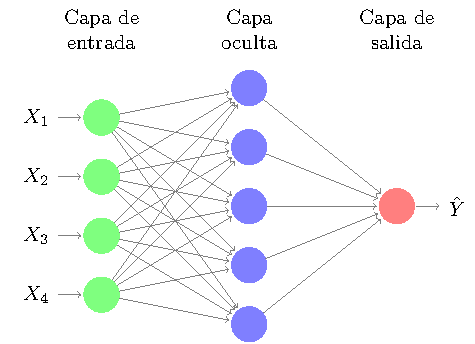
\includegraphics[width=0.8\linewidth]{figuras/neuralNetwork.pdf}
	\caption*{Fuente: elaboración propia, con base en\\ \url{http://www.texample.net/tikz/examples/neural-network/}}
\end{figure}

La capa de entrada recibe las variables explicativas del modelo, de forma análoga con un modelo lineal. La capa de salida es similar a la variable dependiente. Al final de un proceso de entrenamiento, esta capa provee una salida estimada, que puede ser interpretada como la respuesta del modelo a las entradas que no han sido observadas por la red. La capa oculta es crítica para un modelado exitoso, debido a que permite capturar las componentes no observadas en un modelo lineal, y se encarga de capturar la correlación entre las entradas y la salida, lo que provee a la red neuronal con una cierta intuición de predicción e inteligencia en el aprendizaje de los patrones de entrada y salida, ayudando a una correcta inferencia en las relaciones de entradas y salidas no vistas, proceso al que se le conoce como generalización. \parencite{sunythesis} 

%\clearpage

\subsubsection{Principios básicos del modelo de redes neuronales}

Se describe el concepto de función de activación, así como la expresión matemática que representa un modelo de RNA.

\paragraph{Función de activación no lineal}
Una función de activación permite limitar la amplitud de la salida de una neurona. En la figura \ref{ann_structure}, cada una de las neuronas en la capa oculta cuenta con una función de activación.\\

La función de activación se caracteriza cuenta con un grado de no linealidad que permite a la red neuronal detectar y posteriormente reproducir patrones no lineales cuando los datos son muy complejos \parencite{sunythesis}. Debido al algoritmo de entrenamiento utilizado en el ajuste de los pesos sinápticos para una RNAs, la diferenciabilidad es la única condición que debe satisfacer una función de activación \parencite{haykin1999neural}.\\

Los ejemplos de funciones continuamente diferenciables más comúnmente utilizadas en RNAs son las funciones sigmoide logística y tangente hiperbólica. La función logística: \[ \phi(x) = \frac{1}{1 + e^{-x}} \] se utiliza comúnmente en los modelos probabilísticos, mientras que la sigmoide tangente hiperbólica: \[ \phi(x) = \frac{e^x - e^{-x}}{e^x + e^{-x}} \] se utiliza habitualmente en los modelos de regresión, sin embargo, esta última es en realidad la función logística reescalada y sumada a una constante.


\paragraph{Expresión para el modelo de redes neuronales}
% Acá mencionar que la capa de salida tiene una función lineal, debido a que la variable de salida no está acotada en un intervalo
Aunque existen varios tipos de RNAs, las de 3 capas de tipo \textit{feedforward} son las más populares y ampliamente utilizadas, como la que se muestra en la figura \ref{ann_structure}. En la ecuación \ref{ann_model} se muestra la representación más general para una RNA \textit{feedforward} de tres capas, con $J$ neuronas en la capa oculta.

\begin{equation}
	Y = f \bigg ( w_0 + \sum_{j=1}^{J} \phi \big ( w_{0j} + \mathbf{w_j}^T \mathbf{x} \big )\bigg )
	\label{ann_model}
\end{equation}

donde $w_0$ denota un término de intercepto en la neurona de salida, $w_{0j}$ el intercepto en la $j$ neurona oculta, $w_j$ denota el peso sináptico de la $j$ neurona oculta hacia la neurona de salida, $\mathbf{w_j} = (w_{1j}, \ldots, w_{nj})$ el vector de todos los pesos sinápticos de la entrada hacia la neurona $j$, y $\mathbf{x} = (x_1, \ldots, x_n)$ el vector de variables de entrada.\\

Finalmente, $\phi$ representa la función de activación de la capa oculta, y $f$ la función de activación de la neurona de salida. Se hace la distinción debido a que $f$ puede ser la función identidad ($f(x) = x$), que se utiliza generalmente en tratamiento de RNAs como modelos de regresión.

% Técnicas para el modelo de redes neuronales
\subsubsection{Pasos para el desarrollo de la red neuronal}
Para llevar a cabo el desarrollo de la red neuronal, de acuerdo con \textcite{sunythesis}, se deben seguir el siguiente conjunto de pasos:

\begin{enumerate}
	\item Escoger el conjunto de variables explicatorias.

	\item Escoger una arquitectura de RNA adecuada.
	
	\item Seleccionar el número de capas ocultas y el número de neuronas en cada capa oculta, e inicializar los pesos de interconexión.
	
	\item Organizar la muestra en orden temporal ascendente, y dividr los datos en tres conjuntos: de entrenamiento (o ajuste de los pesos), de validación, y de prueba.
	
	\item Utilizar un software para obtener el modelo.
	
	\item Evaluar el desempeño de pronóstico del modelo y comparar con otros modelos lineales y no lineales.
	
	\item Repetir los pasos 3-6 hasta que se alcance el mínimo error de pronóstico sobre el conjunto de validación (el mínimo de la medida de error cuadrático medio).
	
	\item Repetir los pasos 2-7 variando la arquitectura de la red hasta que se alcance un mínimo del error global.
	
	\item Decidir si deben añadirse o removerse variables explicatorias.
	
	\item Finalmente, repetir los pasos 1-9 hasta que se alcance el mínimo error a través de las combinaciones de variables de entrada.
\end{enumerate}


\subsubsection{Elementos técnicos de la red neuronal}
Se describen algunos aspectos relacionados con el entrenamiento y evaluación de la red neuronal.

\paragraph{Normalización de los datos} Para el trabajo se utiliza el logaritmo del tipo de cambio como variable dependiente del modelo, y debido a que se utiliza la función sigmoide tangente hiperbólica, es necesario normalizar los datos de entrada y salida en un rango adecuado, correspondiente al intervalo $(-1, 1)$. Citando a LeCun (1993), cada variable de entrada debe ser preprocesada de tal forma que su valor medio sobre todo el conjunto de entrenamiento esté cercano a cero, o bien, sea pequeño en comparación con su desviación estándar, esto permite acelerar el proceso de aprendizaje de la red neuronal. \parencite{haykin1999neural}.\\

En el trabajo se realiza una normalización de los datos sustrayendo la media de cada una de las variables explicativas y dividiendo por la desviación estándar de la muestra completa (180 observaciones).

\paragraph{Determinación de la arquitectura}
Esta tarea consiste en determinar el número de capas en la red neuronal y el número de elementos en cada capa, lo que determina el número de pesos sinápticos a ser determinados. De acuerdo con \textcite{sunythesis}, seleccionar estos parámetros depende del problema en particular que se desee resolver, debido a que no existe un método teórico sólido que permita seleccionar los mismos.\\

En este trabajo se utiliza una arquitectura de interconexión de cada una de las neuronas con todas las neuronas de la siguiente capa, y se utiliza una arquitectura de una capa oculta, que de acuerdo con el teorema de aproximación universal descrito en \textcite{haykin1999neural}, es suficiente para que una red neuronal artificial compute una aproximación uniforme a un conjunto de entrenamiento representado por el conjunto de entradas\footnote{En \textcite[209]{haykin1999neural} se puede encontrar una descripción completa del teorema.}.\\

En cuanto a la cantidad de neuronas de la capa oculta, se escoge en base a las medidas de error de pronóstico tanto dentro como fuera de la muestra, y finalmente se escogen dos arquitecturas finales para realizar el pronóstico, con ocho y nueve neuronas en su capa oculta.

%Citando a \textcite{haykin1999neural}, el problema con redes neuronales de una sola capa oculta es que las neuronas tienden a interactuar entre sí de forma global, y en situaciones complejas, esta interacción hace difícil mejorar la aproximación en un punto sin empeorarla en otro, mientras que con dos capas ocultas, el proceso de aproximación de curvas se vuelve más manejable.


\paragraph{Algoritmo de entrenamiento}

El algoritmo utilizado para entrenar a la red neuronal se conoce como \textit{backpropagation}, que provee un método computacionalmente eficiente para el ajuste de los pesos sinápticos. La razón por la que este algoritmo adopta este nombre es porque la red es entrenada utilizando los valores de salida deseados, así es posible obtener una medida de error desde la salida, y dicho error es propagado hacia atrás para la modificación (o aprendizaje) de los pesos sinápticos.\\

En este trabajo se utiliza una variante del algoritmo conocida como \textit{resilient backpropagation} (en concreto RPROP+), que modifica los pesos de la red neuronal para encontrar un mínimo local de la función de error. Para esto, el algoritmo computa un gradiente de la función de error respecto a los pesos sinápticos ($dE_{rr}/d\mathbf{w}$) para encontrar una raíz, y en particular, los pesos se modifican en dirección opuesta a las derivadas parciales hasta alcanzar un mínimo local con una cierta medida de tolerancia.

\paragraph{Mínimo global}
En general, no se puede demostrar que el algoritmo de propagación hacia atrás converja, y no hay criterios bien definidos para detener su operación. En su lugar, existen criterios razonables con mérito práctico para terminar el ajuste de pesos. Para formular dichos criterios es necesario pensar en términos de las propiedades de un mínimo local, o global, de la superficie de error \parencite{haykin1999neural}. En este trabajo se utiliza un umbral para las derivadas parciales de la función de error como criterio de parada para el entrenamiento de la red neuronal.\\

En la aplicación de modelos no lineales (como la red neuronal empleada) se tiene la dificultad de que difícilmente se puede saber si se obtuvo un mínimo global en la estimación, porque puede estar enmascarado por muchos mínimos locales con relaciones matemáticas cercanas. Para evitar la introducción de este problema es necesario repetir la estimación utilizando distintos pesos sinápticos iniciales y aleatorios, y finalmente guardar la mejor estimación.



\paragraph{Tamaño de la muestra}
Las RNAs con más observaciones pueden detectar estructuras más complejas y manejar las irregularidades en los datos más efectivamente para alcanzar mayor precisión en el modelado. En este trabajo se utiliza una muestra relativamente larga de 180 observaciones (mensuales de enero de 2001 a diciembre de 2015) para aplicar en la estimación y validación de la red neuronal.



% Finalmente la especifiación del modelo
\subsubsection{Especificación del modelo}

Se utiliza un modelo macroeconómico no lineal $\Phi$ de la forma: 

\[	s_t = \Phi (M_t) + \epsilon_t \]

donde $s_t$ es el logaritmo natural del tipo de cambio $spot$ sobre los meses de observación, y $M_t$ es un vector de variables macroeconómicas, es decir, la oferta relativa de dinero, el ingreso relativo, el diferencial de la tasa de interés, y el diferencial de inflación esperada de largo plazo; $\epsilon_t$ es un término de error aleatorio.\\

La especificación exacta del modelo utilizado es la siguiente:

\begin{equation}
s_t = f(X_{1t}, X_{2t}, X_{3t}, X_{4t}) + \epsilon_t
\label{annModel}
\end{equation}

donde $f$ representa la aproximación de la red neuronal a los datos.\\

% Nuevamente, el pronóstico fuera de la muestra se realiza utilizando las observaciones de las variables explicativas del modelo.

En la figura \ref{fig:ann_monetary9} se muestra el diagrama final de la arquitectura de la red neuronal artificial utilizada para el pronóstico del tipo de cambio, en donde \textit{s} representa el logaritmo natural del tipo de cambio, \textit{m} representa la oferta relativa de dinero, \textit{i} el diferencial de tasas de interés, \textit{y} el diferencial de ingreso real e \textit{inf} el diferencial de inflación esperada.

\begin{figure}[ht]
	\centering
	\caption{Estructura de la red neuronal artificial utilizada para pronóstico}
	\label{fig:ann_monetary9}
	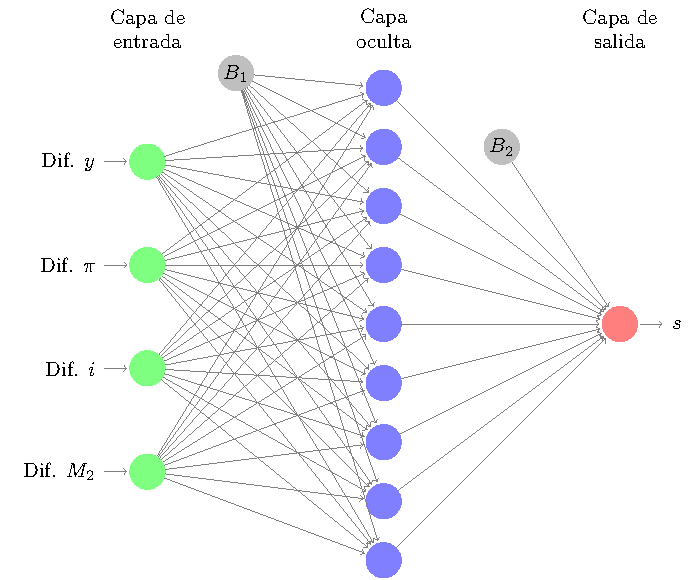
\includegraphics[width=0.8\linewidth]{figuras/spec_ann.pdf}
	\caption*{Fuente: elaboración propia.}
\end{figure}


\subsection{Método de Garson para interpretación de los pesos sinápticos}
Debido a que no existe una interpretación clara de los pesos sinápticos de la red neuronal se utiliza el método de Garson, que identifica la importancia relativa de las variables explicativas para una variable de respuesta de la red neuronal deconstruyendo los pesos del modelo.\\

La idea básica es que la importancia relativa (o fuerza de de asociación) de una variable explicativa para una respuesta específica puede ser determinada identificando todos las conexiones ponderdadas entre los nodos de interés, esto es, se identifican todos los pesos sinápticos que pasan de una entrada específica hacia la capa oculta y finalmente hacia la salida. Finalmente, se obtiene un único valor para cada variable explicativa, que describe la relación con la variable de respuesta de la red neuronal.

% Como se evaluará el modelo: a través de las medidas de pronóstico fuera de la muestra

\subsection{Evaluación del modelo}
Para evaluar el desempeño de los modelos de pronóstico se utilizarán algunas pruebas de especificación dentro de la muestra. El propósito de este trabajo es evaluar el desempeño fuera de la muestra de la red neuronal y compararla con otros modelos. Para cumplir este propósito se guardan las últimas 36 observaciones de la muestra para realizar el pronóstico con los distintos modelos y finalmente contrastar los resultados de acuerdo con las medidas obtenidas.\\

% Una cualidad excepcional de las RNAs es la flexibilidad en la construcción de modelos econométricos, sin embargo, un exceso de flexibilidad puede provocar un problema de sobreajuste (\textit{overfitting}, como se conoce en la literatura) en la red neuronal. Cuando una red neuronal presenta este problema, esta no puede inferir el proceso real de generación de los datos, y afecta negativamente la calidad de los pronósticos.

En este trabajo se utilizan los valores observados de las variables explicativas en los modelos para el pronóstico del tipo de cambio fuera de la muestra, tal como en el trabajo de \textcite{meese1983empirical}, con el objetivo de evaluar la capacidad de inferencia de la RNA sobre los datos.

\subsubsection{Medidas de precisión del pronóstico fuera de la muestra}

La medida de desempeño más importante en una RNA utilizada para pronóstico es la precisión de predicción para observaciones fuera de la muestra. Prácticamente se mide el grado de precisión con el error de pronóstico, que es la diferencia entre el valor observado y el pronosticado.\\

En este trabajo se utiliza como medida de precisión la raíz del error cuadrático medio (RMSE, por sus siglas en inglés), la raíz del error cuadrático medio porcentual (RMSPE), y el Porcentaje de Puntos de Inflexión Correctamente Pronosticados (PERC, por sus siglas en ingleś). El RMSE se puede definir como:

\begin{equation}
	\mathrm{RMSE} = \sqrt{\frac{1}{T} \sum_{t=1}^{T} (Y_t^s - Y_t^a)^2}
	\label{rmsedef}
\end{equation}

donde $Y_t^s$ es el valor estimado (o pronosticado), $Y_t^a$ es el valor observado, y $T$ el número de períodos de pronóstico en los datos. Asimismo, siguiendo la misma notación, el RMSPE se puede definir como: 

\begin{equation}
\mathrm{RMSE} = \sqrt{\frac{1}{T} \sum_{t=1}^{T} (\frac{Y_t^s - Y_t^a}{Y_t^a})^2}
\label{rmspedef}
\end{equation}

El indicador PERC se enfoca en la dirección del pronóstico más que en la precisión de los pronósticos, y sirven para indicar si el modelo puede predecir de forma precisa si el tipo de cambio subirá o bajará en el siguiente período, aunque no necesariamente indique la cantidad. Puede definirse como sigue: 

\begin{equation}
	\mathrm{PERC} = \frac{T_p + T_n}{T}
	\label{percdef}
\end{equation}

donde $T_p$ y $T_n$ representan el número de predicciones correctas con signo positivo y negativo, respectivamente, y $T$ el número total de predicciones.
